% -*- mode: LaTeX; TeX-PDF-mode: t; -*-
% LaTeX path to the root directory of the current project, from the directory in which this file resides
% and path to econtexPaths which defines the rest of the paths like \FigDir
\providecommand{\econtexRoot}{}\renewcommand{\econtexRoot}{.}
\providecommand{\econtexPaths}{}\renewcommand{\econtexPaths}{\econtexRoot/Resources/econtexPaths}
% The \commands below are required to allow sharing of the same base code via Github between TeXLive on a local machine and Overleaf (which is a proxy for "a standard distribution of LaTeX").  This is an ugly solution to the requirement that custom LaTeX packages be accessible, and that Overleaf prohibits symbolic links
\providecommand{\econtex}{\econtexRoot/Resources/texmf-local/tex/latex/econtex}
\providecommand{\econark}{\econtexRoot/Resources/texmf-local/tex/latex/econark}
\providecommand{\econtexSetup}{\econtexRoot/Resources/texmf-local/tex/latex/econtexSetup}
\providecommand{\econtexShortcuts}{\econtexRoot/Resources/texmf-local/tex/latex/econtexShortcuts}
\providecommand{\econtexBibMake}{\econtexRoot/Resources/texmf-local/tex/latex/econtexBibMake}
\providecommand{\econtexBibStyle}{\econtexRoot/Resources/texmf-local/bibtex/bst/econtex}
\providecommand{\econtexBib}{economics}
\providecommand{\economics}{\econtexRoot/Resources/texmf-local/bibtex/economics}
\providecommand{\notes}{\econtexRoot/Resources/texmf-local/tex/latex/handout}
\providecommand{\handoutSetup}{\econtexRoot/Resources/texmf-local/tex/latex/handoutSetup}
\providecommand{\handoutShortcuts}{\econtResourexRoot/Resources/texmf-local/tex/latex/handoutShortcuts}
\providecommand{\handoutBibMake}{\econtexRoot/Resources/texmf-local/tex/latex/handoutBibMake}
\providecommand{\handoutBibStyle}{\econtexRoot/Resources/texmf-local/bibtex/bst/handout}

\providecommand{\FigDir}{\econtexRoot/Figures}
\providecommand{\CodeDir}{\econtexRoot/Code}
\providecommand{\DataDir}{\econtexRoot/Data}
\providecommand{\SlideDir}{\econtexRoot/Slides}
\providecommand{\TableDir}{\econtexRoot/Tables}
\providecommand{\ApndxDir}{\econtexRoot/Appendices}

\providecommand{\ResourcesDir}{\econtexRoot/Resources}
\providecommand{\rootFromOut}{..} % APFach back to root directory from output-directory
\providecommand{\LaTeXGenerated}{\econtexRoot/LaTeX} % Put generated files in subdirectory
\providecommand{\econtexPaths}{\econtexRoot/Resources/econtexPaths}
\providecommand{\LaTeXInputs}{\econtexRoot/Resources/LaTeXInputs}
\providecommand{\LtxDir}{LaTeX/}
\providecommand{\EqDir}{Equations} % Put generated files in subdirectory

% \owner determines where links to online content go
% llorracc is Chris Carroll's personal version
% econ-ark is the Econ-ARK/REMARK version
%\providecommand{\owner}{llorracc}
\providecommand{\owner}{econ-ark}

\documentclass[pdflatex]{beamer}
\usepackage{ifthen}
\newboolean{Web}\setboolean{Web}{false}
\usepackage{econark}
\providecommand{\texname}{Bprep-Slides}%

% Can't read in Bprep.sty because some packages conflict with Beamer
% So need to redefine everything here

\usepackage{econark}
\usepackage{\econtexShortcuts}
\usepackage{\LaTeXInputs/\texname}

\setboolean{showPageHead}{false}

\usepackage{amsmath,amssymb,rotating,subfigure}
\usepackage{verbatim,moreverb,graphicx}
\usepackage{wasysym}
\usepackage{dcolumn}
\usepackage{cancel}
%\renewcommand{\LtxDir\EqDir}{\econtexRoot/Equations}
\providecommand{\FigsRaw}{\econtexRoot/Code/Python/Figures}
\providecommand{\CodeDir}{\econtexRoot/Code}
\providecommand{\CalibrationDir}{\econtexRoot/Calibration}
\providecommand{\TableDir}{\econtexRoot/Tables}
\providecommand{\ApndxDir}{\econtexRoot/Appendices}
\providecommand{\Ex}{\mathbb{E}}

\usepackage{bibentry}
\usepackage[backend=bibtex,style=authoryear]{biblatex}
\addbibresource{Bprep.bib}


\mode<presentation>
{
  \usetheme{Warsaw}
  % or ...
  \setbeamercovered{transparent}
}

%\beamerdefaultoverlayspecification{<+->}

%\setbeamertemplate{navigation symbols}{}  % Take away navigation symbols

\usetheme{Warsaw}

\setbeamersize{text margin left=3mm}
\setbeamersize{text margin right=3mm}


%_____________ Opening slide _______________________

\title[Bowel Prep Improvements]{A Patient-centered Framework for Health Systems Engineering in Gastroenterology}
\author[Hsu]{Lawrence Hsu}
\institute[JHU]{Johns Hopkins University}
\date[\today]{September 12, 2019  \\ \medskip \medskip \medskip \href{https://econ-ark.org/}{\small Powered By} \\ 
\includegraphics[width=0.5in]{\econtexRoot/Resources/econ-ark-logo-small.png}}

\begin{document}

\begin{frame}[plain]
  \titlepage
\end{frame}


\section{Introduction}
\subsection{Background}

\begin{frame}
\frametitle{Rationale of Improving Bowel Preparation}

\begin{itemize}
\item Inpatient Colonoscopy Scheduled $\Rightarrow$ Bowel Prep Began
\item What happens with {\it inadequate} bowel preps (clinically)? 
\begin{itemize}
\item Adverse Events (\cite{Almadi2018-lx})
\item Delayed or Repeated Procedures (\cite{Ness2001-ff})
\item Negative Patient Outcome (\cite{Garber2019-rw})
\end{itemize}
\medskip
\item Improvement Goal: Medicine Alternation
\end{itemize}

\end{frame}

\subsection{Control Features}
\begin{frame}
\frametitle{Elements Impacting Bowel Prep Results}

\begin{itemize}
\item Socioeconomic Status \& Gender (\cite{Yadlapati2018-kg})
\item Age (\cite{Chung2009-kt})
\item Marriage Status (\cite{Lebwohl2010-ti})
\item Complications:
\begin{itemize}
  \item Diabetes Mellitus (\cite{Reilly2004-tz})
  \item Chronic Constipation (\cite{Hautefeuille2014-yy})
  \item Cirrhosis (\cite{Ness2001-ff})
\end{itemize}
\item {\bf Poor Compliance} (\cite{Almadi2018-lx})
\end{itemize}

\medskip
\begin{itemize}
  \item Phase 1 Control before Medication Differences
\end{itemize}
\end{frame}

\begin{frame}
\frametitle{Individualized Characteristics}
% Table 1
%\documentclass[8pt, letterpaper]{article}
%\begin{document}
\hypertarget{Characteristics of patients pre- and post-intervention to improve inpatient colonoscopy bowel preparation}{}
 \begin{table}
  \centering
  \caption{Characteristics of patients pre- and post-intervention to improve inpatient colonoscopy bowel preparation}
  \label{table:character}
    \begin{tiny}
    \begin{tabular}{lllr} \hline
    & Pre-intervention & Post-intervention & p-value \\
    & (n=120) & (n=129) & \\ \hline
    Individual factors & & & \\
    \ \ Age, mean (sd) & 58.8 (17.34) & 57.8 (17.5) & 0.65\\
    \ \ Male & 61 (50.8) & 63 (48.8) & 0.75 \\
    \ \ Race, non-white & 58 (48.3) & 76 (58.9) & 0.10 \\
    \ \ Primary team medicine service & 113 (94.2) & 113 (87.6) & 0.07 \\
    Indication & & & 0.85 \\
    \ \ Diarrhea, colitis & 20 (16.7) & 25 (19.4) & \\
    \ \ Fecal transplant & 1 (0.8) & 3 (2.3) & \\
    \ \ Abdominal pain & 2 (1.7) & 4 (3.1) & \\
    \ \ Anemia & 16 (13.3) & 18 (14.0) & \\
    \ \ Colon cancer & 14 (11.7) & 14 (10.9) & \\
    \ \ Constipation & 2 (1.7) & 0 & \\
    \ \ Gastrointestinal bleeding & 55 (45.8) & 54 (41.9) & \\
    \ \ Inflammatory bowel disease & 10 (8.3) & 11 (8.5) & \\
    Systems factors & & & \\
    Hourly inpatient occupancy, mean (range) & 86.75 (85.61, 87.97) & 90.32 (88.88, 90.88) & $<$ 0.001 \\ \hline
    \multicolumn{4}{l}{\textbf{Data are presented as Number (\%) unless otherwise noted}}\\
    \multicolumn{4}{l}{\textbf{Sd: standard deviation}}\\
    \end{tabular}
    \end{tiny}
 \end{table}
%\end{document} 
\end{frame}

\section{Process Changes}
\subsection{Protocol for Bowel Prep}
\begin{frame}
\frametitle{Initiated Protocol for Bowel Prep}
    \begin{figure}
        \centerline{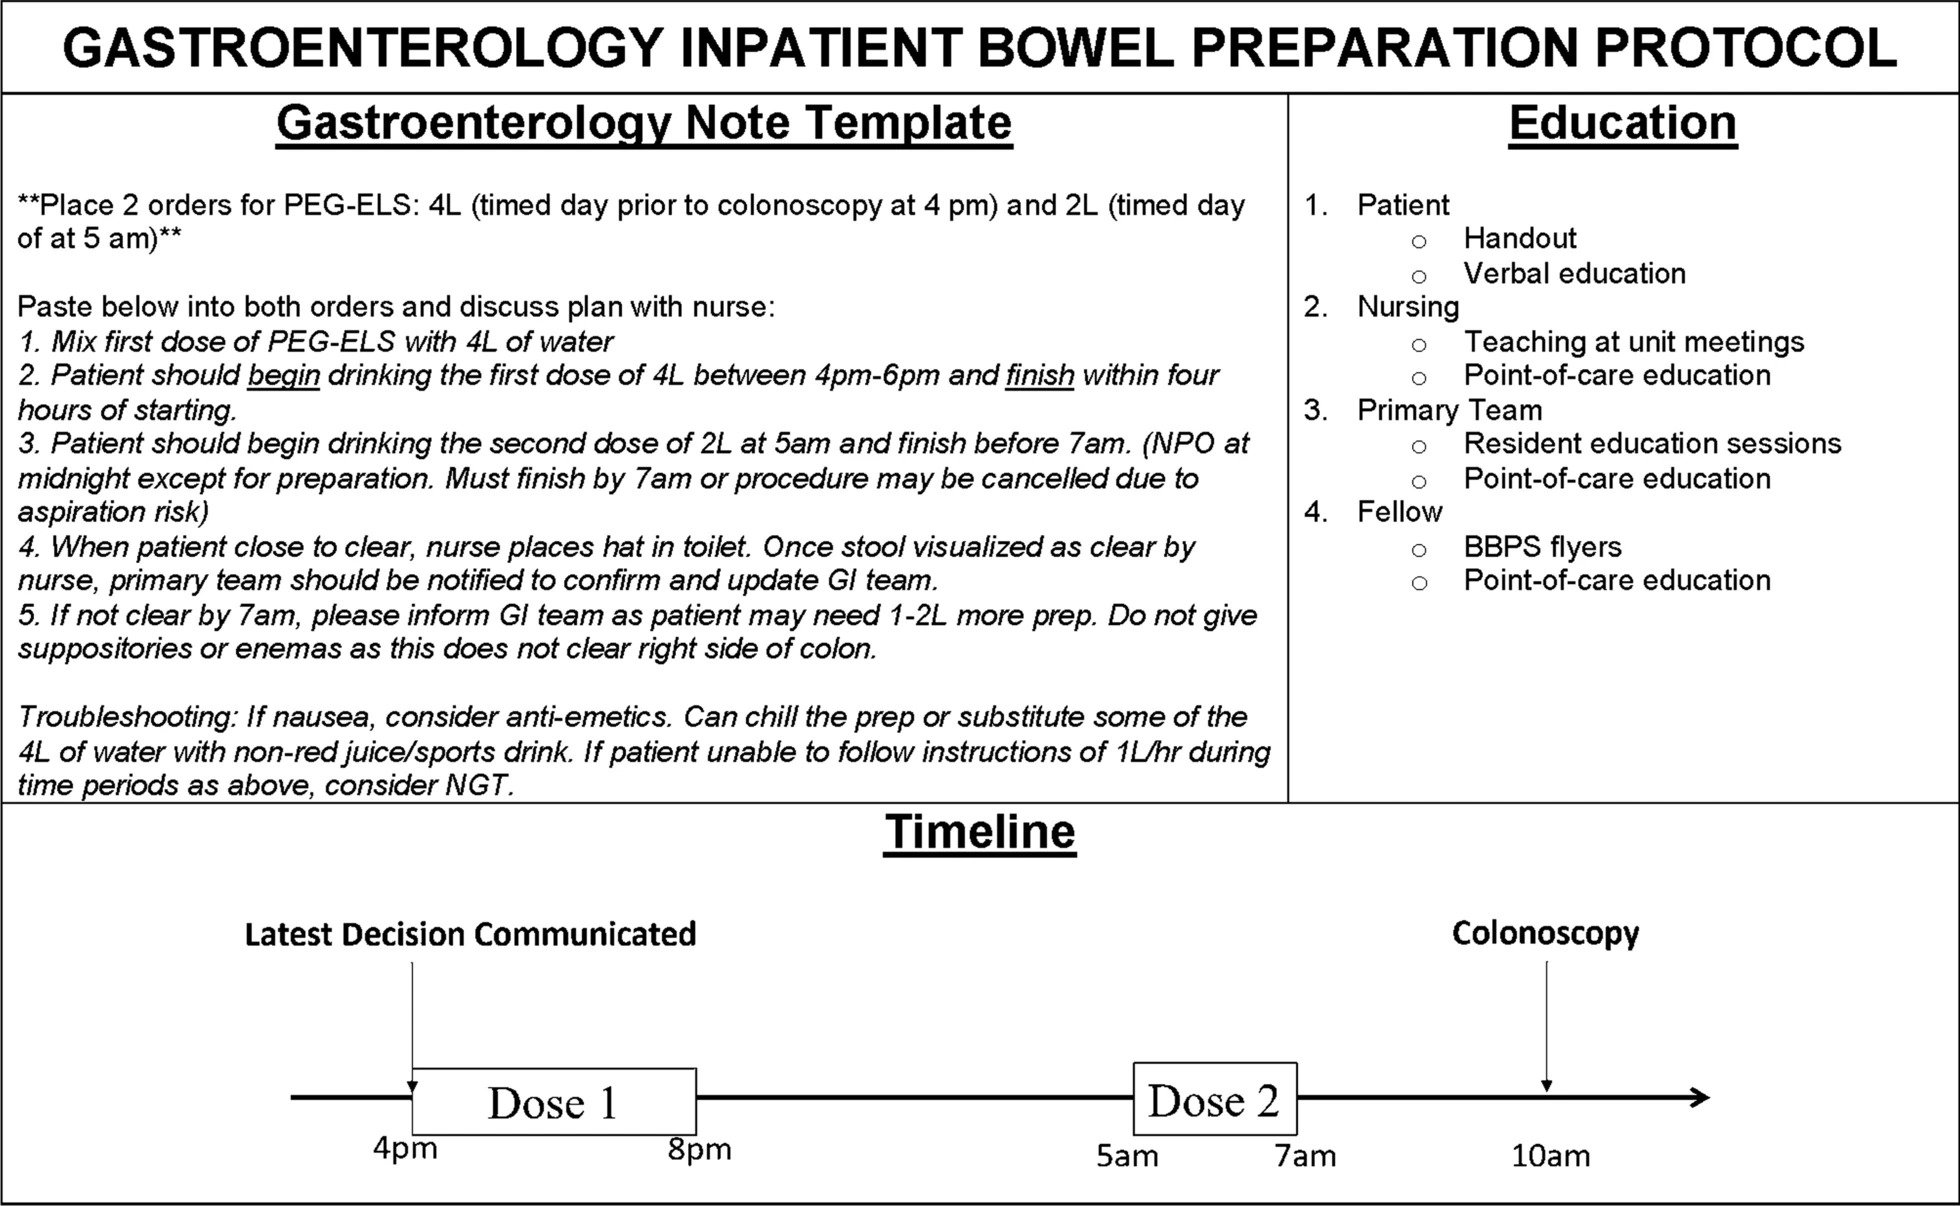
\includegraphics[width=0.75\linewidth]{\FigDir/Figure2.jpg}}
    \end{figure}
\end{frame}

\begin{frame}
\frametitle{How the Medication Change Work}

\begin{itemize}
\item Lower GI Bleed (\cite{Saltzman2015-ir})
\item Ref: \cite{American_Society_of_Anesthesiologists_Committee2011-sw}
\medskip
\item Additional Requirement: {\bf Patient Education} (\cite{Lai2009-xr})
\medskip
\item The old way: one dose with 4-L of polyethylene glycol (PEG)
\item Renewed method: 4-L $+$ 2-L doses of glycol-electrolyte solution
\begin{itemize}
  \item Verbal Communication by 4 p.m. of the Decision
  \item 4-L Dose between 4 p.m. and 6 p.m. Prior to Colonoscopy
  \item 2-L Dose between 5 a.m. and 7 a.m. On the Colonoscopy Date
\end{itemize}
\end{itemize}
\end{frame}

\subsection{How the Flow Chart Changes}
\begin{frame}
\frametitle{Workflow Identifying Medication Alteration}
    \begin{figure}
        \centerline{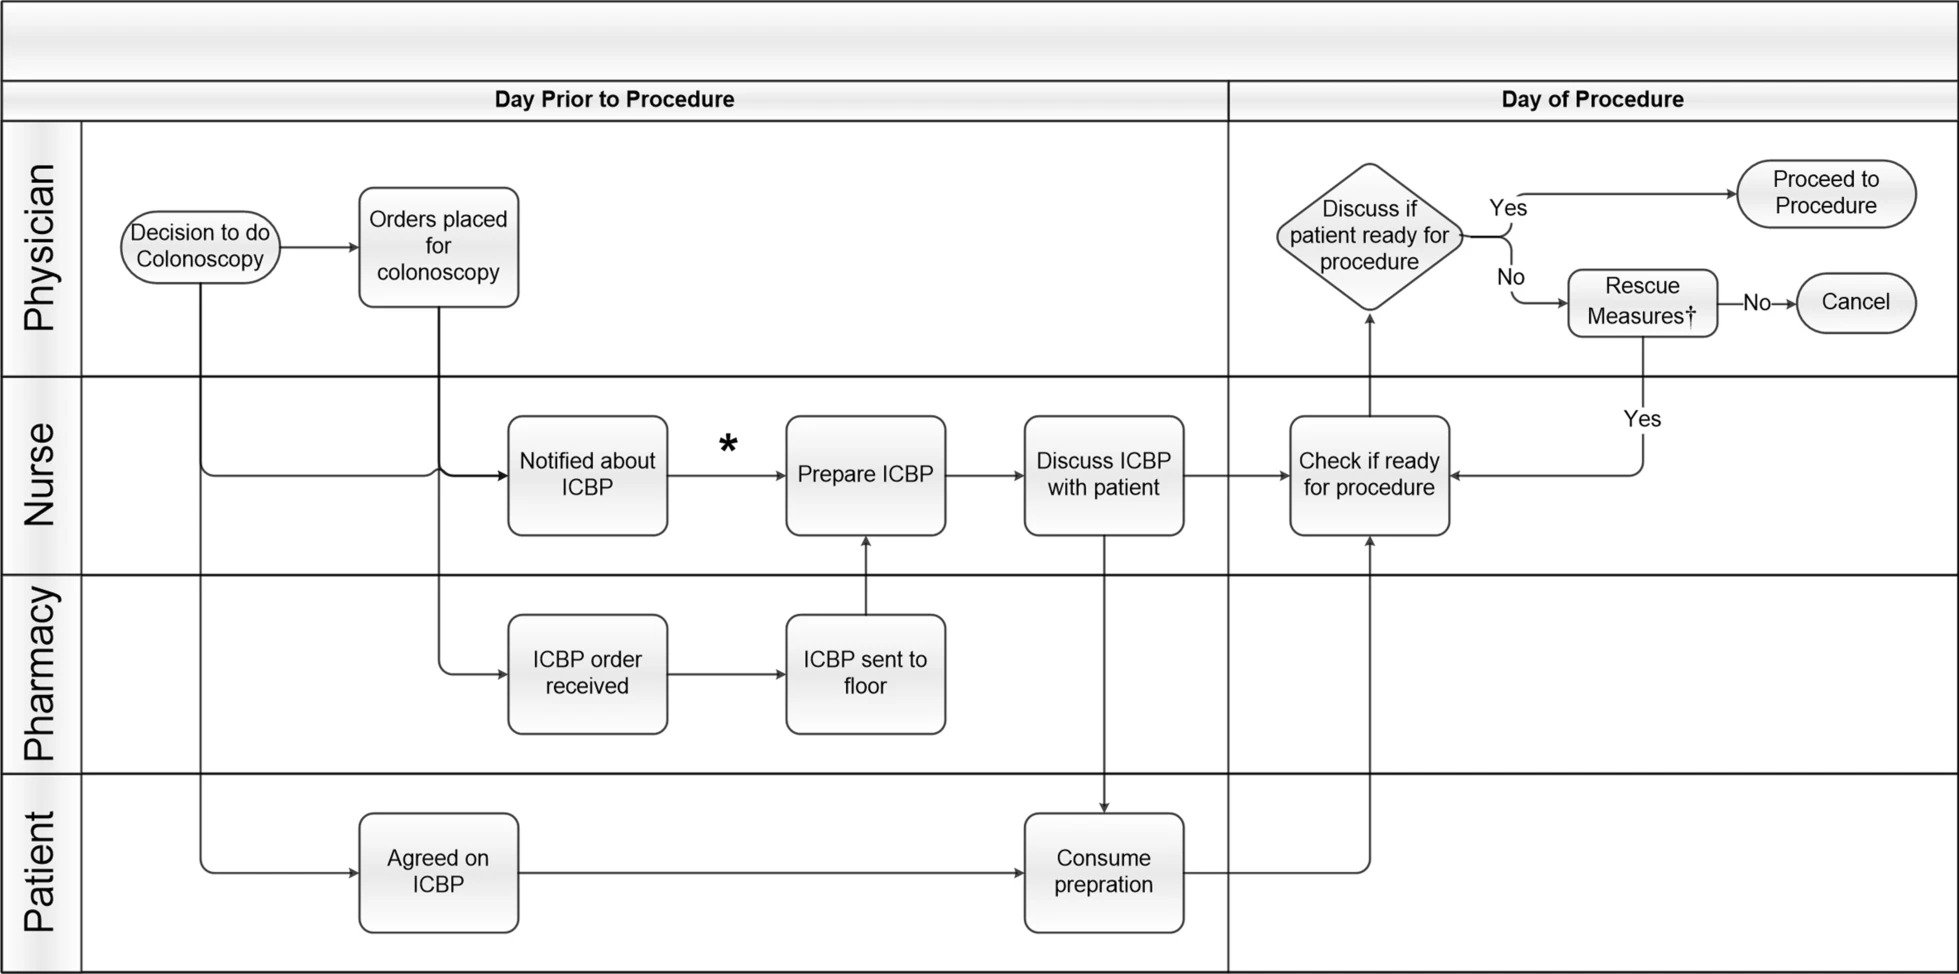
\includegraphics[width=0.75\linewidth]{\FigDir/Figure1.jpg}}
    \end{figure}
\end{frame}

\section{Modeling the Improvements}
\subsection{Capturing the BBPS Score}
\begin{frame}
\frametitle{Runchart Capturing Preparation Score}
\begin{itemize}
    \item Boston Bowel Preparation Score (BBPS): Visibility by Radiology
    \item Creating Runcharts for Trending (\cite{Perla2011-dp})
\end{itemize}
    \begin{figure}
        \centerline{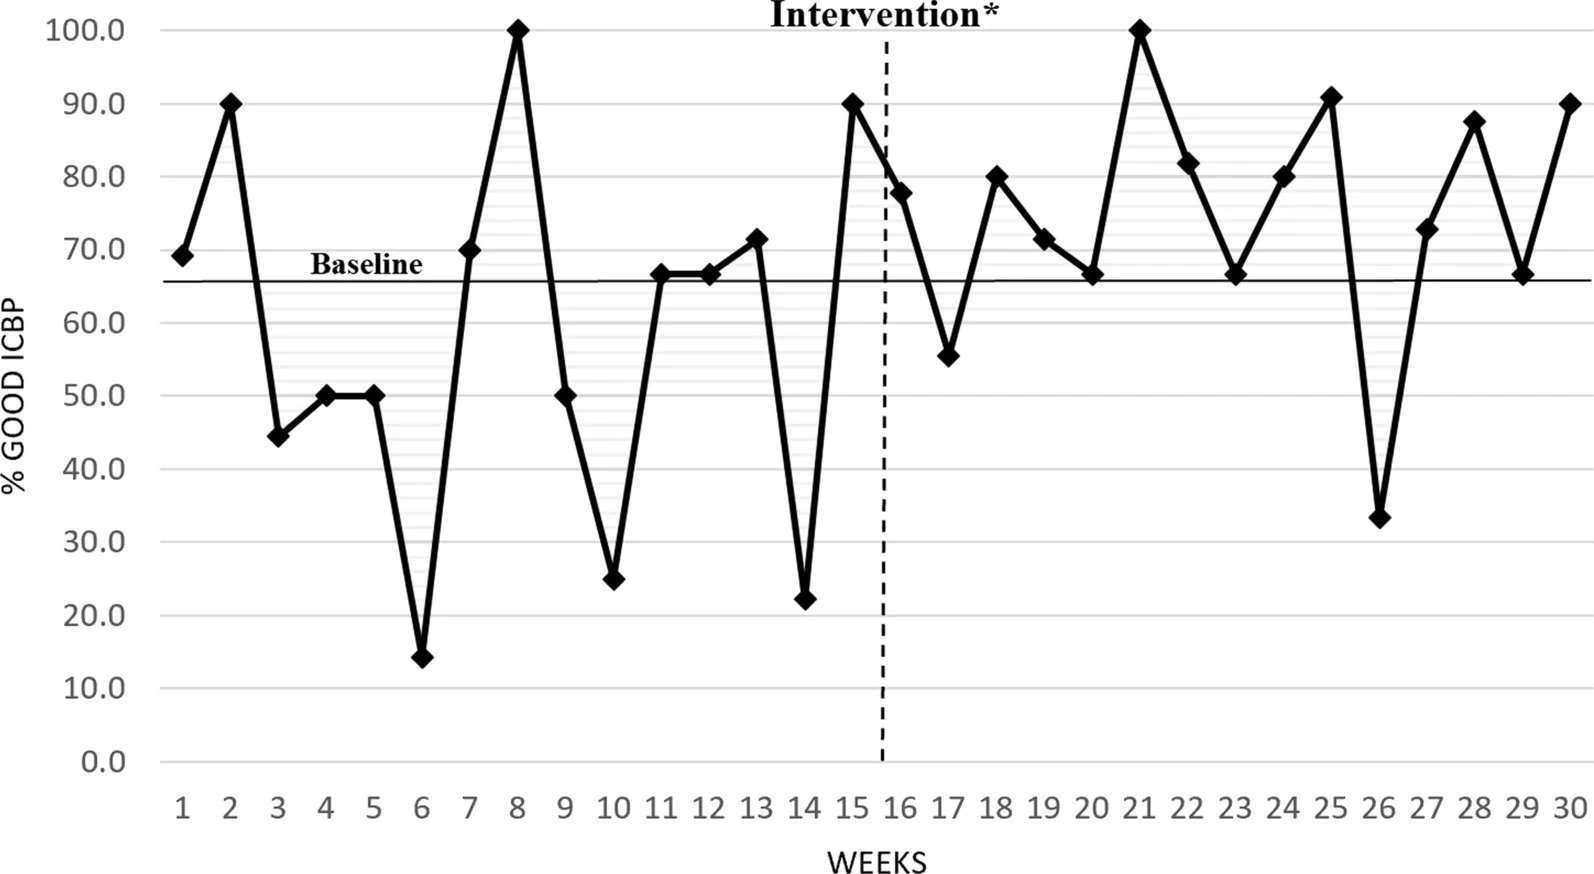
\includegraphics[width=0.6\linewidth]{\FigDir/Figure3.jpg}}
    \end{figure}
\end{frame}

\subsection{Model Factors (Tests Applied)}
\begin{frame}
\frametitle{Study of Intervention and Analysis}
\begin{itemize}
  \item Good ICBP: Procedure delayed, but bowel prep successful 
  \item Ideal ICBP: Procedure on time, and bowel prep successful
\end{itemize}
\medskip
\begin{itemize}
    \item Pre- and Post-Intervention: T-test, Wilcoxon Sum Rank Test
    \item Categorical Variables: Chi-square Test, Fisher's Exact Test
    \item Linear Splines for Time Estimates (\cite{Johnson2014-nm})
\end{itemize}

\end{frame}

\subsection{Modeling Results}
\begin{frame}
\frametitle{Results of the Analysis}
\begin{itemize}
    \item Improvements on Both ICBP Status
    \item Improvements on Length of Stay
\end{itemize}
% Table 2
%\documentclass[8pt, letterpaper]{article}
%\begin{document}
\hypertarget{Estimates from generalized linear model for adequate bowel preparations and length of stay before and after the intervention in unadjusted and adjusted models}{}
 \begin{table}
  \centering
  \caption{Estimates from generalized linear model for adequate bowel preparations and length of stay before and after the intervention in unadjusted and adjusted models}
  \label{table:estimates}
    \begin{tiny}
    \begin{tabular}{llll} \hline
    \textbf{Study Outcome} & \textbf{Pre vs. Post} & \textbf{Unadjusted Model} & \textbf{Adjusted Model} \\
     & & \textbf{Relative Risk (Pre/Post)} & \textbf{Relative Risk (Pre/Post)}\\
     & & \textbf{[95\% Confidence Interval]} & \textbf{[95\% Confidence Interval]}\\ \hline
    Good$^{\sharp}$ ICBP & 60.8\% vs. 74.4\% & 1.873* & 1.947* \\
     & & [1.093,3.211] & [1.025,3.697] \\
    Ideal$^{\ddag}$ ICBP & 53.3\% vs. 69.0\% & 1.947* & 1.901* \\
     & & [1.160,3.266] & [1.024,3.531] \\ \hline
     & & \textbf{Ratio of Means (Pre/Post)} & \textbf{Ratio of Means (Pre/Post)}\\
     & & \textbf{[95\% Confidence Interval]} & \textbf{[95\% Confidence Interval]}\\ \hline
    Mean Length of Stay, Days & 8 vs. 6 & 0.759 & 0.852 \\
     & & [0.538,1.069] & [0.617,1.179] \\ \hline
    \multicolumn{4}{l}{\textbf{Adjusted model includes average weekly occupancy. ICBP: inpatient colonoscopy bowel preparations.}}\\
    \multicolumn{4}{l}{\textbf{$\sharp$ Good: Colonoscopy delayed and adequate bowel preparation when performed. }}\\
    \multicolumn{4}{l}{\textbf{$\ddag$ Ideal: Colonoscopy not delayed and adequate bowel preparation when performed. * p$<$0.05}}\\
    \end{tabular}
    \end{tiny}
 \end{table}
%\end{document} 
\end{frame}

\subsection{Conclusion and Limitations}
\begin{frame}
\frametitle{Conclusion and Limitations}
\begin{itemize}
  \item This is only a single-center QI study with high patient volume
  \item Length of Stay estimation: multipliers \& flow uncertainties
\end{itemize}
\medskip
\begin{itemize}
    \item Difficult to control certain comorbidities
    \item The unknown status we want to know: {\bf Past Failed Bowel Preps}
    \item Compliance measurements (with qualitative input)
\end{itemize}
\medskip
\begin{itemize}
  \item Still, this is a piece of literature showing the necessity to alter golden-standard medication for bowel prep (PEG-GES)
\end{itemize}
\end{frame}

\begin{frame}
\frametitle{Qualitative Input: Next Steps}
\begin{figure}
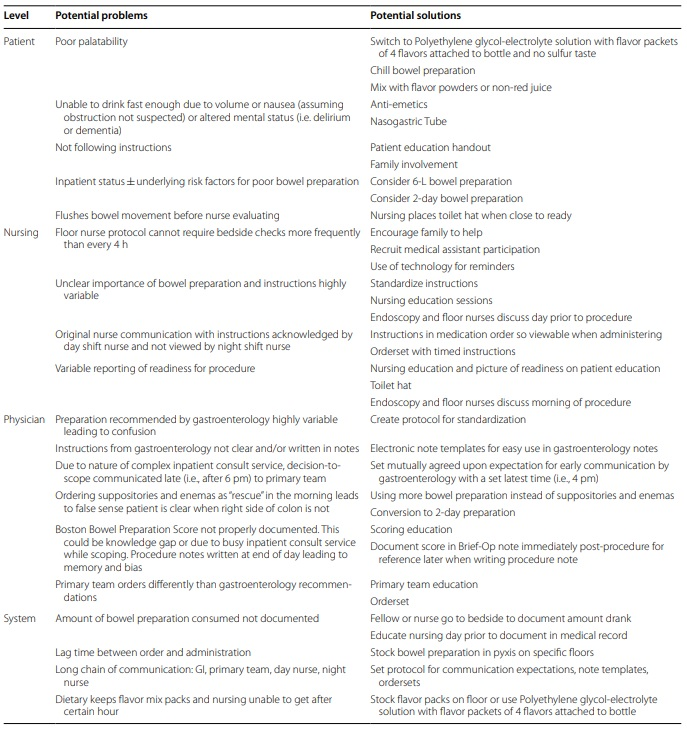
\includegraphics[width=0.5\linewidth]{./Tables/Table_3.jpg}
\end{figure}
\end{frame}

\end{document}

% Local Variables:
% TeX-master-file: t
% eval: (setq TeX-command-list  (assq-delete-all (car (assoc "BibTeX" TeX-command-list)) TeX-command-list))
% eval: (setq TeX-command-list  (assq-delete-all (car (assoc "Biber"  TeX-command-list)) TeX-command-list))
% eval: (setq TeX-command-list  (remove '("BibTeX" "%(bibtex) ../LaTeX/%s"    TeX-run-BibTeX nil t :help "Run BibTeX") TeX-command-list))
% eval: (setq TeX-command-list  (remove '("BibTeX"    "bibtex ../LaTeX/%s"    TeX-run-BibTeX nil (plain-tex-mode latex-mode doctex-mode ams-tex-mode texinfo-mode context-mode)  :help "Run BibTeX") TeX-command-list))
% eval: (setq TeX-command-list  (remove '("BibTeX" "bibtex ../LaTeX/%s"    TeX-run-BibTeX nil t :help "Run BibTeX") TeX-command-list))
% eval: (add-to-list 'TeX-command-list '("BibTeX" "bibtex LaTeX/%s" TeX-run-BibTeX nil t                                                                              :help "Run BibTeX") t)
% eval:  (add-to-list 'TeX-command-list '("BibTeX" "bibtex LaTeX/%s" TeX-run-BibTeX nil (plain-tex-mode latex-mode doctex-mode ams-tex-mode texinfo-mode context-mode) :help "Run BibTeX") t)
% TeX-PDF-mode: t
% TeX-file-line-error: t
% TeX-debug-warnings: t
% LaTeX-command-style: (("" "%(PDF)%(latex) %(file-line-error) %(extraopts) -output-directory=./LaTeX %S%(PDFout)"))
% TeX-source-correlate-mode: t
% TeX-parse-self: t
% TeX-parse-all-errors: t
% eval: (cond ((string-equal system-type "darwin") (progn (setq TeX-view-program-list '(("Skim" "/Applications/Skim.app/Contents/SharedSupport/displayline -b %n LaTeX/%o %b"))))))
% eval: (cond ((string-equal system-type "gnu/linux") (progn (setq TeX-view-program-list '(("Evince" "evince --page-index=%(outpage) LaTeX/%o"))))))
% eval: (cond ((string-equal system-type "gnu/linux") (progn (setq TeX-view-program-selection '((output-pdf "Evince"))))))
